%%% LaTeX Template: Article/Thesis/etc. with colored headings and special fonts
%%%
%%% Source: http://www.howtotex.com/
%%% Feel free to distribute this template, but please keep to referal to http://www.howtotex.com/ here.
%%% February 2011
%%%
%%% Modified January 2016 by CDM

%%%  Preamble
\documentclass[11pt,letterpaper]{article}
\usepackage[margin=1.0in]{geometry}
\usepackage[T1]{fontenc}
\usepackage[bitstream-charter]{mathdesign}
\usepackage[latin1]{inputenc}					
\usepackage{amsmath}						
\usepackage{xcolor}
\usepackage{cite}
\usepackage{hyphenat}
\usepackage{graphicx}
\usepackage{float}
\usepackage{subfigure}
\usepackage{sectsty}
\usepackage[compact]{titlesec} 
\usepackage[tablegrid]{vhistory}
\usepackage{pbox}
\allsectionsfont{\color{accentcolor}\scshape\selectfont}

%%% Definitions
\definecolor{accentcolor}{rgb}{0.0,0.0,0.5} 
\newcommand{\teamname}{Team C}
\newcommand{\productname}{Language Pronounciation Assisting App}
\newcommand{\coursename}{CSE 4317: Senior Design II}
\newcommand{\semester}{Fall 2017}
\newcommand{\docname}{Detailed Design Specification}
\newcommand{\department}{Department of Computer Science \& Engineering}
\newcommand{\university}{The University of Texas at Arlington}
\newcommand{\authors}{Josue C.\\Ali S.\\Nowreen J.\\Xiwen D.\\Kristen R.}

%%% Headers and footers
\usepackage{fancyhdr}
	\pagestyle{fancy}						% Enabling the custom headers/footers
\usepackage{lastpage}	
	% Header (empty)
	\lhead{}
	\chead{}
	\rhead{}
	% Footer
	\lfoot{\footnotesize \Team C \ - \Fall 2017}
	\cfoot{}
	\rfoot{\footnotesize page \thepage\ of \pageref{LastPage}}	% "Page 1 of 2"
	\renewcommand{\headrulewidth}{0.0pt}
	\renewcommand{\footrulewidth}{0.4pt}

%%% Change the abstract environment
\usepackage[runin]{abstract}			% runin option for a run-in title
%\setlength\absleftindent{30pt}			% left margin
%\setlength\absrightindent{30pt}		% right margin
\abslabeldelim{\quad}	
\setlength{\abstitleskip}{-10pt}
\renewcommand{\abstractname}{}
\renewcommand{\abstracttextfont}{\color{accentcolor} \small \slshape}	% slanted text

%%% Start of the document
\begin{document}

%%% Cover sheet
{\centering \huge \color{accentcolor} \sc \textbf{\department \\ \university} \par}
\vspace{1 in}
{\centering \huge \color{accentcolor} \sc \textbf{\docname \\ \coursename \\ \semester} \par}
\vspace{0.5 in}
\begin{figure}[h!]
	\centering
   	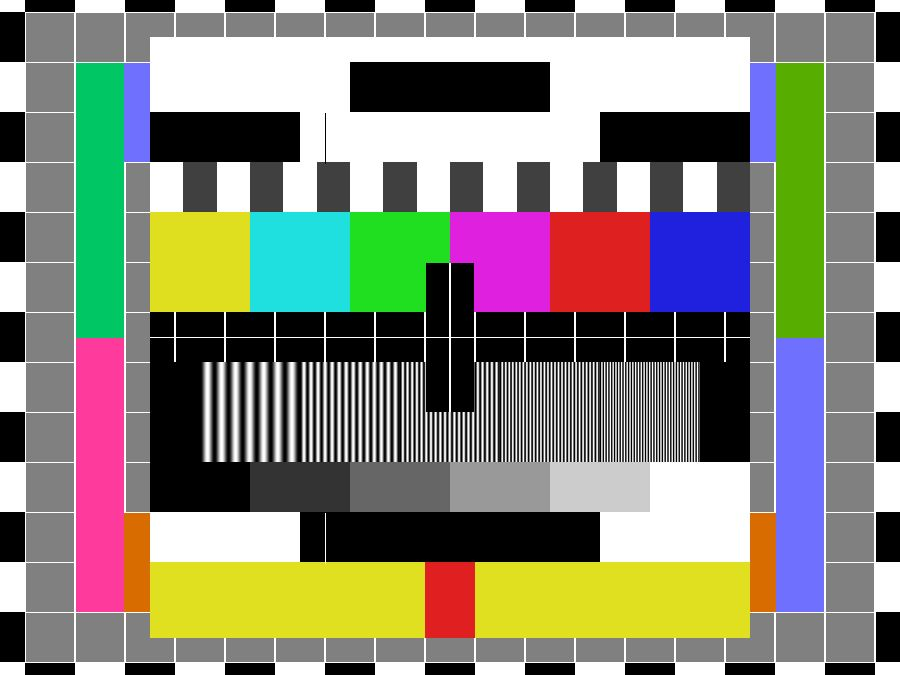
\includegraphics[width=0.60\textwidth]{images/test_image}
\end{figure}
\vspace{0.5 in}
{\centering \huge \color{accentcolor} \sc \textbf{\teamname \\ \productname} \par}
\vspace{0.5 in}
{\centering \large \sc \textbf{\authors} \par}
\newpage


%\vspace{1 in}
%\centerline{January 13th, 2012}
%\newpage

%%% Revision History
\begin{versionhistory}
  	\vhEntry{0.1}{10.22.2017}{GH}{document creation}
\end{versionhistory}
\newpage

%%% Table of contents
\setcounter{tocdepth}{2}
\tableofcontents
\newpage

%%% List of figures and tables (optional)
\listoffigures
\listoftables
\newpage

%%% Document sections
\section{Introduction}
This section describes the purpose, use and intended user audience for the Language Pronunciation App.
The Language Pronunciation App is an application that helps users improve their pronunciation of phonetically difficult words.


Users will be able to visualize their distance to the ``perfect`` phonetic pronunciation of a word.

\section{Architecture Overview}
In order to minimize the burden of processing on the individual clients that utilize our system the application takes a lightweight-client approach to the traditional client-server application.

\begin{figure}[h!]
	\centering
 	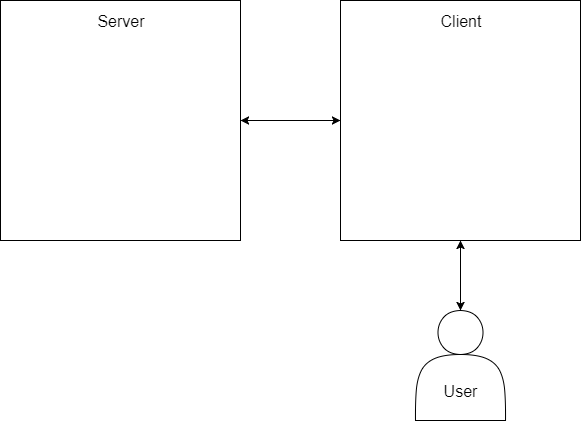
\includegraphics[width=0.60\textwidth]{images/layers}
 \caption{A high-level data-flow diagram for our application}
\end{figure}

\subsection{Client Layer}
The client will function as the HMI between our system and the user. It consists of a UI, and methods by which it may communicate with the server.

\subsection{Server Layer}
The server will function as the work-horse for the application. It's purpose is to host the visualization function which will map an input of word, audio to a distance metric in the form of x, y co-ordinates.

\newpage
\section{Subsystem Definitions \& Data Flow}
\begin{figure}[h!]
	\centering
 	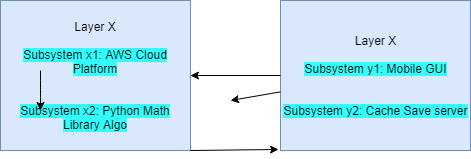
\includegraphics[width=\textwidth]{images/data_flow_syed}
 \caption{The data flow diagram for our app}
\end{figure}

\newpage
\section{Client Layer Subsystems}
\subsection{Client Subsystem}
The client layer subsystem will display the UI of the application. 
It has a XY graph and a dot calculator.
It has a button for record the voice of the users

\begin{figure}[h!]
	\centering
 	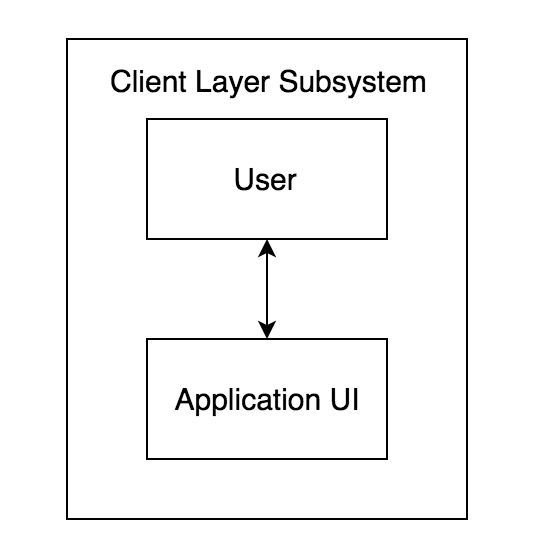
\includegraphics[width=0.60\textwidth]{images/subsystem_client.png}
 \caption{Client subsystem diagram}
\end{figure}

\subsubsection{Assumptions}
The users press the record button, it will be recorded the sound and display the accurate dot.

\subsubsection{Responsibilities}
The Client Layer Subsystem will send the user's voice to the application, and interaction with user. And it will display a dot on the application UI.
The Client Layer should display all information to user. And receive user's request.

\subsubsection{Subsystem Interfaces}
Each of the inputs and outputs for the subsystem are defined here. Create a table with an entry for each labelled interface that connects to this subsystem. For each entry, describe any incoming and outgoing data elements will pass through this interface.

\begin {table}[H]
\caption {Client Subsystem interfaces} 
\begin{center}
    \begin{tabular}{ | p{1cm} | p{6cm} | p{3cm} | p{3cm} |}
    \hline
    ID & Description & Inputs & Outputs \\ \hline
    \#1 & XY Graph & \pbox{3cm}{N/A} & \pbox{3cm}{Red dot}  \\ \hline
    \#2 & Voice Record Button & \pbox{3cm}{User's sound} & \pbox{3cm}{N/A}  \\ \hline
    \end{tabular}
\end{center}
\end{table}

\newpage
\section{Server Layer Subsystems}
\subsection{Server Subsystem}
The system records the users voice sound and send it to sever. 
Sever compare the sound with the database and calculate the difference and send back to the application.

\begin{figure}[h!]
	\centering
 	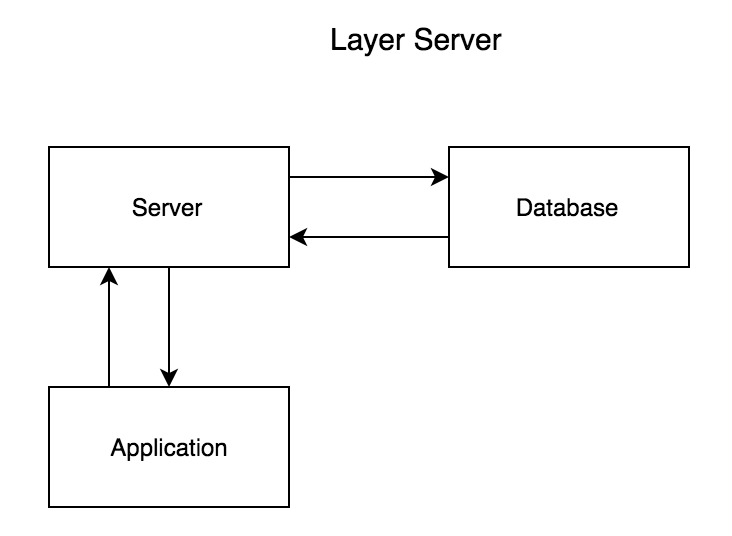
\includegraphics[width=0.60\textwidth]{images/subsystem_server}
 \caption{Server subsystem diagram}
\end{figure}

\subsubsection{Assumptions}
The Server receive the user's voice data and compare data with the standard voice data from the database.

\subsubsection{Responsibilities}
The application sends the voice data to the server.
The sever get data from the database and calculate the difference, then send the information back.
The application records the user's sound, and send to the server, and when sever received the user's voice data, then compare data with the standard voice data from the database. The server send back the \% difference to the application.

\subsubsection{Subsystem Interfaces}
\begin {table}[H]
\caption {Server Subsystem interfaces} 
\begin{center}
    \begin{tabular}{ | p{1cm} | p{6cm} | p{3cm} | p{3cm} |}
    \hline
    ID & Description & Inputs & Outputs \\ \hline
    \#1 & Display the graph dot by calculate the difference of the voice words & \pbox{3cm}{Voice Words} & \pbox{3cm}{Graph Dot}  \\ \hline
    \end{tabular}
\end{center}
\end{table}

\newpage
\section{Appendix A}
\input{tex/appendix_a.tex}
\newpage

%%% References
\bibliographystyle{plain}
\bibliographystyle{reference/IEEEtran_custom}
\bibliography{reference/refs}{}

\end{document}
